Voici un programme écrit avec le logiciel Scratch.

\begin{center}
\begin{scratch}[scale=1,print]
    \blockinit{quand \greenflag est cliqué}
    \blockpen{effacer tout}
    \blockmove{aller à x: \ovalnum0 y: \ovalnum0}
    \blockmove{s’orienter à \ovalnum{90} degrés}    
    \blockrepeat{répéter \ovalnum{4} fois}
    {
    \blockpen{stylo en position d’écriture}
    \blockmove{avancer de \ovalnum{10}}
    \blockpen{relever le stylo}
    \blockmove{avancer de \ovalnum{10}}    
    \blockmove{tourner \turnright{} de \ovalnum{90} degrés}
    }
\end{scratch}
\end{center}

\begin{enumerate}
    \item Représenter la figure obtenue lorsque le programme est exécuté. On prendra $1$ mm pour $1$ pixel.
    \item Marie souhaite obtenir la figure ci-dessous où chaque tiret mesure $10$ pixels et est séparé 
    du précédent de $10$ pixels. Quelle(s) modification(s) doit-elle apporter au programme ?
    \begin{center}
        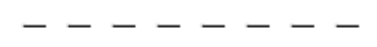
\includegraphics[width=0.6\textwidth]{./images/2022-g3-ex4-img1.png}
    \end{center}
    \item 
    \begin{enumerate}
        \item Léo souhaite modifier le programme donné pour que l’on obtienne la figure ci-dessous.
        
        Quelle(s) modification(s) doit-il apporter au programme de départ ?
        \begin{center}
            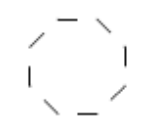
\includegraphics[width=0.2\textwidth]{./images/2022-g3-ex4-img2.png}
        \end{center}
        \item Quel type de transformation géométrique permet de passer d’un tiret à un autre ?        
    \end{enumerate}
\end{enumerate}